\chapter{Implementing drivel}\label{ch:implementation}

This chapter describes implementation efforts, challenges, and noteworthy information for implementers, including deployment steps and practical considerations such as traffic shaping.
\Cref{sec:tech-stack} gives an overview of the technology stack, languages, and libraries used in the implementation, with a particular focus on the changes made to the preexisting lyrebird project \cite{lyrebird} to support \drivel{}. This section also describes the environment in which the protocol was developed and tested.
\Cref{sec:parameters} outlines the process for choosing concrete cryptographic parameters, focusing on the trade-offs between security and traffic volume.
\Cref{sec:protocol-design} presents a high-level description of the \drivel{} protocol, followed by a detailed explanation of how handshake messages could be fragmented to enhance traffic shaping capabilities.
\Cref{sec:impl-architecture} describes how the protocol design was mapped to the actual software components, including noteworthy architectural changes and cryptographic interfaces.
\Cref{sec:deployment} provides practical guidance for the deployment and use of the system, with attention to real-world integration barriers.
Finally, \cref{sec:challenges-learnings} discusses the key challenges encountered during development and how they were addressed.

\section{Technology Stack and Environment} \label{sec:tech-stack}

The implementation created as part of this thesis is available via GitLab. It consists of two parts: A fork of the lyrebird project \cite{lyrebird} where the \drivel{} pluggable transport is implemented\footnote{See \url{https://gitlab.ethz.ch/himarc/lyrebird-pq-obfs}}, and a larger repository which includes a testing and benchmarking framework, analysis code and TeX sources of this document\footnote{See \url{https://gitlab.ethz.ch/himarc/thesis-quantumsafe-fep}}.

\paragraph{Structure of the lyrebird Fork and Dependencies}

The \drivel{} implementation, like the other six pluggable transports in the lyrebird repository, is written in Go. The lyrebird repository contains several Go modules:
\begin{itemize}
    \item \texttt{cmd} implements general pluggable transport logic and represents the program entry point.
    
    \item \texttt{common} contains various useful implementations such as cryptographically secure random number generation (CSRNG), deterministic random bit generation (DRBG), logging, probability distributions, filter objects to prevent replay attacks, SOCKS5 implementation, etc. These implementations may be reused outside of the lyrebird repository. 
    
    \item \texttt{internal} contains implementations that are only reusable within lyrebird. The upstream repository only contained an x25519 and \textsf{Elligator2}~\cite{CCS:BHKL13} implementation in this module.
    
    \item \texttt{transports} finally has submodules for each pluggable transport that each implement a common interface used by the \texttt{cmd} module. 
\end{itemize}

During the course of this thesis, the \texttt{internal} module was significantly refactored and extended. Furthermore, a new submodule \texttt{transports/drivel} was added to the \texttt{transports} module, based on a copy of the \texttt{transports/obfs4} module. We refer readers to \cref{sec:impl-architecture} for details about these changes.

External Go dependencies required for \drivel{} and not specific to other pluggable transports are limited to the following modules and versions:
\begin{itemize}
    \item \gopkgref{filippo.io/edwards25519}{v1.1.0} for easier handling of elliptic-curve cryptography,
    
    \item \gopkgref{gitlab.com/yawning/edwards25519-extra}{v0.0.0-20231005122941-2149dcafc266} for its implementation of \textsf{Elligator2}~\cite{CCS:BHKL13},
    
    \item \gopkgref{github.com/dchest/siphash}{v1.2.3} for the pseudorandom function employed in the DRBG,
    
    \item \gopkgref{github.com/open-quantum-safe/liboqs-go}{v0.0.0-20250119172907-28b5301df438} as a Go wrapper around the C library \texttt{liboqs} which provides many KEM implementations,
    
    \item \gopkgref{gitlab.torproject.org/tpo/anti-censorship/pluggable-transports/goptlib}{v1.6.0} for handling arguments passed to the pluggable transport, and
    
    \item \gopkgref{golang.org/x/crypto}{v0.32.0} for its implementation of some elliptic-curve operations, HKDF and NaCl secretbox.
\end{itemize}

Other than \texttt{liboqs-go}, all of these dependencies were present in the upstream repository and required for \obfsfour{}.

In addition to the Go modules above, \drivel{} also depends on the \href{https://github.com/open-quantum-safe/liboqs}{liboqs} C library, compiled statically from source during the build process. This archive is then included in a local build of \texttt{liboqs-go}, removing the need for lyrebird users to install \texttt{liboqs} separately.

However, the inclusion of C code also means that a fully static compilation of the forked lyrebird repository was not possible anymore in Go's default build process. The upstream repository accomplished this via the use of the flag \texttt{CGO\_ENABLED}. Instead, the final executable now requires the following dynamically linked libraries to be present on the system:
\begin{itemize}
    \item \texttt{linux-vdso.so.1}
    \item \texttt{libresolv.so.2}
    \item \texttt{libpthread.so.0}
    \item \texttt{libc.so.6}
    \item \texttt{/lib64/ld-linux-x86-64.so.2}
\end{itemize}

To run end-to-end tests, the official bridge setup guide \cite{tor-bridge-setup} refers, among other options, to a Docker container \cite{tor-bridge-docker}.
We were able to adapt the container's configuration to use our forked repository and our modified build process (which now includes building \texttt{liboqs}) instead of the upstream version. The required dynamic libraries were already present on the system, demonstrating that deployment should not be hindered by our modifications to the dependencies and executable.

\paragraph{Testing and Benchmarking}

To perform unit and integration tests of the different software components, Go's built-in support for testing and benchmarking files was used. We have transferred all existing test cases for \obfsfour{} and extended them to include all new software components, and cover all enabled KEM/OKEM combinations.

In particular, cryptographic operations within \drivel{} are tested using positive and negative test cases on different levels. Unit tests verify the submodule's correctness, and integration tests simulate entire handshakes, including (de-)serialization of messages to and from byte strings.

The tests include a small variant that performs fewer tests of randomized functions, making a trade-off between execution time and completeness. All tests pass for the entire forked repository, also in their more extensive variant.

Benchmarks are also performed on multiple levels, including single KEM and OKEM operations (key generation, encapsulation, and decapsulation), as well as the execution of a complete simulated handshake. The latter benchmark allows a direct comparison to the corresponding \obfsfour{} benchmark. Furthermore, profiling can easily be performed to identify bottlenecks in the benchmark's performance and to quantify contributions to its memory consumption.

The results were collected and analyzed in Python and R. Further discussion of the results follows in \cref{ch:results}.

\section{Choosing Parameter Sets} \label{sec:parameters}

\paragraph{Supported KEMs and OKEMs}
We begin with an overview of all supported KEMs and OKEMs in our implementation, including their parameter sets and corresponding NIST security levels 1, 3, and 5.

The following OKEMs are available for each NIST security level:
\begin{itemize}
    \item ML-Kemeleon, as in \cite{irtf-cfrg-kemeleon-00}, based on ML-KEM-512 (level 1), ML-KEM-768 (level 3), and ML-KEM-1024 (level 5)
    \item Unmodified FrodoKEM \cite{NISTPQC-R3:FrodoKEM20}, concretely FrodoKEM-640-AES (level 1), FrodoKEM-976-AES (level 3), and FrodoKEM-1344-AES (level 5)
    \item Unmodified Classic McEliece, as in \cref{sec:obfuscating-classic-mceliece}, concretely Classic-McEliece-348864 (level 1), Classic-McEliece-460896 (level 3), as well as Classic-McEliece-6688128, Classic-McEliece-6960119, and Classic-McEliece-8192128 (all three claiming level 5)
    \item $\feo[\mathsf{HQC}, E_\mathsf{HQC}]$, as in \cref{sec:obfuscating-hqc}, concretely based on HQC-128 (level 1), HQC-192 (level 3), and HQC-256 (level 5)
\end{itemize}

In addition, it is possible to use the implementation of x25519 and \textsf{Elligator2}~\cite{CCS:BHKL13} as an OKEM, but as this OKEM would not be resistant against quantum-computers, we only include it for the purposes of performance comparisons with \obfsfour{}.

For the selection of a KEM, the implementation supports the following for each NIST security level:
\begin{itemize}
    \item BIKE \cite{NISTPQC-R4:BIKE22}, concretely BIKE-L1 (level 1), BIKE-L3 (level 3), and BIKE-L5 (level 5)
    \item Streamlined NTRU Prime \cite{NISTPQC-R3:NTRUPrime20}, concretely sntrup761 (level 2)
    \item Unobfuscated variants for each OKEM listed above, except Classic-McEliece
\end{itemize}

Again, it is also possible to use a KEM based on x25519, which is not quantum-safe.

\paragraph{Disabled KEMs and OKEMs}

Due to the fact that our implementation relies on AES to instantiate the symmetric encryption component of \drivel{}, and to reduce the amount of options to consider in the following sections, we support only AES variants of FrodoKEM, even though SHAKE version are offered by \texttt{liboqs}.
Similarly, but motivated also by a desire for a smaller traffic volume during the key exchange and a desire for smaller buffer sizes, Classic McEliece has been disabled as a KEM (though it remains available as an OKEM).
FrodoKEM variants using SHAKE, as well as unobfuscated Classic McEliece KEMs, could easily be re-enabled if so desired.

\paragraph{Selected Combinations}

Although \drivel{} can be instantiated with any choice of KEM or OKEM listed above, most combinations lead to inconsistent security levels or excessive message sizes. To reduce the number of combinations to a sensible amount, \cref{tab:drivel-params} defines a total of 12 sets of KEM/OKEM combinations, four for each of the NIST security levels 1, 3, and 5.

For the selection of parameter sets, we can observe that Classic-McEliece-6960119, and Classic-McEliece-8192128 will not selected as an OKEM because they achieve no higher NIST security level than Classic-McEliece-6688128 but use longer ciphertexts.
Further, we did not use sntrup761 as a KEM even though it would offer a 30\% reduction in size compared to BIKE-L1, as no other NTRU Prime parameter sets are available for NIST levels 3 and 5.

These parameter sets prioritize the selection of combinations that lead to the smallest required total handshake traffic, excluding padding.
\begin{table}
    \centering  \footnotesize
    \begin{tabular}{@{} L{0.1\textwidth-\tabcolsep} | L{0.16\textwidth-2\tabcolsep} L{0.17\textwidth-2\tabcolsep} L{0.32\textwidth-2\tabcolsep} R{0.11\textwidth-2\tabcolsep} R{0.14\textwidth-\tabcolsep} @{}}
    NIST Security\newline Level & Parameter Set\newline Name & KEM\newline Component & OKEM\newline Component & Total Traffic & First Fragment \\ \hline
    \multirow{4}{*}{Level 1} & drivel-L1a & ML-KEM-512 & ML-Kemeleon-512 & 2 541 & 893 \\
     & drivel-L1b & BIKE-L1 & ML-Kemeleon-512 & 4 087 & 893 \\
     & drivel-L1c & ML-KEM-512 & FEO-HQC-128 & 6 097 & 4 449 \\
     & drivel-L1d & ML-KEM-512 & Classic-McEliece-348864 & 1760 & 112 \\ \hline
    \multirow{4}{*}{Level 3} & drivel-L3a & ML-KEM-768 & ML-Kemeleon-768 & 3 620 & 1 268 \\
     & drivel-L3b & BIKE-L3 & ML-Kemeleon-768 & 7 546 & 1 268 \\
     & drivel-L3c & ML-KEM-768 & FEO-HQC-192 & 11 346 & 8 994 \\
     & drivel-L3d & ML-KEM-768 & Classic-McEliece-460896 & 2 524 & 172 \\ \hline
    \multirow{4}{*}{Level 5} & drivel-L5a & ML-KEM-1024 & ML-Kemeleon-1024 & 4 890 & 1 674 \\
     & drivel-L5b & BIKE-L5 & ML-Kemeleon-1024 & 12 030 & 1 674 \\
     & drivel-L5c & ML-KEM-1024 & FEO-HQC-256 & 17 653 & 14 437 \\
     & drivel-L5d & ML-KEM-1024 & Classic-McEliece-6688128 & 3 440 & 224
    \end{tabular}
    \caption[
        Definitions of parameter sets for \drivel{}, used in later experiments.
    ]{
        Definitions of parameter sets for \drivel{}, used in later experiments.
        Total traffic shows the combined number of bytes required across all handshake messages, excluding padding. First fragment denotes the size in bytes of just OKEM ciphertext and a 16 byte PRF value and thus illustrates the minimum amount of valid data required before the bridge may reply.
    }
    \label{tab:drivel-params}
\end{table}

Notably, HQC is not included as an unobfuscated KEM in any parameter set, due to its larger public key size compared to both ML-KEM and BIKE. Due to its more conservative assumptions, but consequently larger public key and ciphertext sizes, FrodoKEM is not included as KEM or OKEM in any parameter set. Depending on the assumptions one is comfortable with, ``a'' parameter sets may be suitable as only one KEM has to remain unbroken, whereas ``b'' can profit from different underlying assumptions for its KEM and OKEM, while ``c'' parameter sets feature a simpler encoding routine. Finally, ``d'' parameter sets employ Classic McEliece as an OKEM directly and require confidence in its pseudorandomness (see \cref{sec:obfuscating-classic-mceliece}), but offer significantly smaller message sizes.

When choosing between ``a'' and ``b'' parameter sets, it is worth considering the likelihood of the following scenario where a censor manages to break just one assumption underlying a used KEM or OKEM.
In an ``a'' parameter set, only the assumptions underlying ML-KEM are relevant, but a break could lead to a complete loss of confidentiality as censors might be able to infer the shared secrets generated in recorded key exchanges, decrypt all corresponding traffic and impersonate the bridge server from then on out.
In an ``b'' parameter set, the use of different underlying assumptions makes a break in any assumption more likely, but breaking only one assumption does not immediately mean a loss of all security guarantees: As an example, a censor that completely breaks an OKEM may impersonate bridge servers and retroactively identify obfuscated key exchanges, but cannot recover the KEM shared secrets and is thus not able to retroactively decrypt recorded traffic.

\section{Protocol Design} \label{sec:protocol-design}

For a definition of the \drivel{} protocol, as we implemented it in the course of this thesis, we refer readers to \cite[Figure~6]{EPRINT:GRSV25}, which served as our primary source.
This section quickly discusses how we chose to instantiate the generic primitives in the above source before diving into a theoretical discussion on proposed improvements to the protocol to better support traffic shaping.

\subsection{Instantiating the Drivel Protocol} \label{ssec:drivel-instance}

The specification of \drivel{} in \cite[Figure~6]{EPRINT:GRSV25} defines a handful of generic cryptographic primitives that need to be instantiated with concrete choices before implementation.
The authors offer some recommendations in \cite[Section~4.2]{EPRINT:GRSV25}.

We instantiate the primitives as follows:
\begin{itemize}
    \item the PRF $F_1$ is instantiated as \textsf{HDKF-Expand} with \textsf{SHA-256} \cite{C:Krawczyk10,rfc5869},
    
    \item the dual-PRF is instantiated as $F_2$ as \textsf{HMAC-SHA-256} \cite{C:BelCanKra96,KraBelCan97}, and
    
    \item the symmetric encryption scheme $SE$ is chosen to be \textsf{AES-256-CTR} with the appropriate key lengths $\keylen_1 = \keylen_2 = 256$ bits and a fixed IV of zero bytes.
\end{itemize}

We differ from the author's recommendations and the protocol specification only in two points:
\begin{enumerate}
    \item We do not use XOR as our one-time secure symmetric encryption scheme, and instead use AES in CTR mode. Using XOR would involve setting $\keylen_1 = \pklen$ and $\keylen_2 = \ctxtlen$, and the outputs of \textsf{HDKF-Expand} (used as $F_1$) are inherently limited to at most 8 160 bytes. This limitation would not affect any of our parameter sets proposed in \cref{sec:parameters}, but would lead to an avoidable loss of flexibility in the choice of KEM.

    \item The literal strings used for domain separation (such as e.g. ``:enckey1'') are prefixed with the string constant ``Drivel'', just as in \obfsfour{}. This cautionary measure helps to guarantee domain separation even in the case of reused keypairs over multiple protocol versions.
\end{enumerate}

\subsection{Discussion on Fragmenting Handshake Messages} \label{ssec:fragmentation}

This section analyzes possibilities to allow for more flexibility in shaping \drivel{} traffic. Avoiding fingerprinting based on certain sizes, directionalities and timing of messages between client and bridge is crucial to evade censors.

\textbf{No changes discussed or proposed in this \cref{ssec:fragmentation} were implemented, or practically evaluated as part of this thesis, but this discussion may be valuable to readers to understand possible future directions of the protocol.}

\paragraph{Fragmentation is Needed}
When deploying \drivel{}, it may be desirable to offer even more flexibility for traffic shaping than \obfsfour{}. In particular, \obfsfour{} sends two messages in its handshake, before fragmenting packets using a customizable message size distribution based on a deterministic pseudorandom number generator and a seed determined by the bridge server.

While \drivel{} also requires two messages to complete the handshake, \obfsfour{} messages range from 141 to 8 192 bytes in length, and \drivel{} message sizes depend on the selected KEM and OKEM. Ignoring the padding for the moment, \cref{tab:frag-msg-sizes} gives an overview of the minimum message sizes required for different combinations of KEM and OKEM in \drivel{}.

\begin{table}
    \centering \footnotesize
    \begin{tabular}{@{} L{0.2\textwidth-\tabcolsep} L{0.33\textwidth-2\tabcolsep} | L{0.3\textwidth-\tabcolsep} @{}}
    KEM with\newline Parameter Sets & OKEM with\newline Parameter Sets & Minimum Sizes (bytes)\newline Level 1 / Level 3 / Level 5 \\ \hline
    
    \multirow{4}{*}[-2.6em]{\shortstack[l]{ML-KEM\\ 512 / 768 / 1024}}
    & Classic-McEliece\newline 348864 / 460896 / 6688128\vspace{0.3em} & 928 / 1 372 / 1 808 \\
    & ML-Kemeleon\newline 512 / 768 / 1024\vspace{0.3em} & 1 709 / 2 468 / 3 258 \\
    & FEO-HQC\newline 128 / 192 / 256\vspace{0.3em} & 5 265 / 10 194 / 16 021 \\
    & FrodoKEM\newline 640 / 976 / 1344\vspace{0.3em} & 10 552 / 16 960 / 23 232 \\ \hline

    \multirow{4}{*}[-2.6em]{\shortstack[l]{BIKE\\ L1 / L3 / L5}}
    & Classic-McEliece\newline 348864 / 460896 / 6688128\vspace{0.3em} & 1 669 / 3 271 / 5 362 \\
    & ML-Kemeleon\newline 512 / 768 / 1024\vspace{0.3em} & 2 450 / 4 367 / 6 812 \\
    & FEO-HQC\newline 128 / 192 / 256\vspace{0.3em} & 6 006 / 12 093 / 19 575 \\
    & FrodoKEM\newline 640 / 976 / 1344\vspace{0.3em} & 11 293 / 18 859 / 26 786 \\ \hline

    \multirow{4}{*}[-2.6em]{\shortstack[l]{HQC\\ 128 / 192 / 256}}
    & Classic-McEliece\newline 348864 / 460896 / 6688128\vspace{0.3em} & 2 377 / 4 710 / 7 485 \\
    & ML-Kemeleon\newline 512 / 768 / 1024\vspace{0.3em} & 3 158 / 5 806 / 8 935 \\
    & FEO-HQC\newline 128 / 192 / 256\vspace{0.3em} & 6 714 / 13 532 / 21 698 \\
    & FrodoKEM\newline 640 / 976 / 1344\vspace{0.3em} & 12 001 / 20 298 / 28 909 \\ \hline

    \multirow{4}{*}[-2.6em]{\shortstack[l]{FrodoKEM\\ 640 / 976 / 1344}} 
    & Classic-McEliece\newline 348864 / 460896 / 6688128\vspace{0.3em} & 9 744 / 15 820 / 21 760 \\
    & ML-Kemeleon\newline 512 / 768 / 1024\vspace{0.3em} & 10 525 / 16 916 / 23 210 \\
    & FEO-HQC\newline 128 / 192 / 256\vspace{0.3em} & 14 081 / 24 642 / 35 973 \\
    & FrodoKEM\newline 640 / 976 / 1344\vspace{0.3em} & 19 368 / 31 408 / 43 184
    \end{tabular}
    \caption[
        Minimum sizes in bytes for the first \drivel{} message without padding depending on the choice of KEM and OKEM
    ]{
        Minimum sizes in bytes for the first \drivel{} message without padding depending on the choice of KEM and OKEM. Each cell contains minimum sizes for NIST security levels 1, 3, and 5.
        In the case of Classic McEliece, specific KEM parameter sets were selected to minimize message sizes while maintaining the targeted security level. The KEM parameter sets are identified in the first two columns.
    }
    \label{tab:frag-msg-sizes}
\end{table}

The concern in this section is that censors may observe particular traffic patterns. In particular, a bridge server never sends a reply before receiving the entire first \drivel{} or \obfsfour{} message in order to avoid probing attacks. This leads to quiet periods which may constitute an identifiable feature of the pluggable transport.

As is obvious from the table, sending the entire first \drivel{} message in full before the bridge responds (after verifying the PRF value at the end of message) leads to a large quiet period. Thus, for all but a few KEM/OKEM combinations, this quiet period would quickly be identifiable. At best, using Classic McEliece or ML-Kemeleon as an OKEM while employing ML-KEM or BIKE as a KEM still yields sizes not exceeding 8 192 bytes but the quiet periods would still be easy to distinguish from e.g. \obfsfour{} traffic.

\paragraph{Desirable Security Properties}
Before discussing the options to mitigate this risk, let us recall one of the advantages \drivel{} has over \obfsfour{}. In \obfsfour{}, censors can retroactively identify handshake packets by verifying the MAC value if the bridge information is leaked, as the MAC it is keyed only with the bridge information. This allows censors to definitively identify clients that had previously connected to a bridge, as well as any future clients connecting to the bridge. This property has been discussed in \cite[Section~6]{CCS:GunSteVei24} and was also recognized earlier by David Fifield in \cite{obfs4-pk-reveal-distinguisher}.

Instead, \drivel{} establishes a shared secret between the client and the bridge in the first message. This shared secret is then used in addition to the bridge information to key the PRF. Censors therefore cannot retroactively identify obfuscated key exchanges with certainty, unless the OKEM private key is leaked. We will refer to this property here as \emph{strong obfuscation} ($\sObf$), as formally defined in \cite{CCS:GunSteVei24}.

For $\drivel$ to maintain its security, it is necessary that:
\begin{itemize}
    \item[a)] the bridge verifies the client's knowledge of the bridge information before sending a reply, and that
    \item[b)] the client's message proving this is indistinguishable from random bits, even given the bridge information and independent proofs from other clients.
\end{itemize}

Violating a) would make the bridge vulnerable to probing attacks by censors that do not know the bridge information. On the other hand, violating b) would trivially break $\sObf$. Both of these outcomes would be undesirable and $\sObfKE$ from \cite{CCS:GunSteVei24} captures both avenues of attack, since the predicate \textsf{Probed} automatically wins the game, and public keys can be revealed when asked to distinguish a simulated from a real transcript in \textsc{ChallExec}, respectively.

Due to the required proof in the client's initial communication alone, it is strictly necessary that the bridge server receive a certain minimum amount of data before it may respond in any way.
To break up the first large \drivel{} message, we could, for example, split it into parts and let the server respond after receiving smaller parts. However, the first such ``fragment'' would need to contain at least a suitable proof that the client knows the bridge information.

\paragraph{An Informal Security Notion}
In order to outline the above requirements a bit more, we can informally define the initial interaction between an adversary and the bridge servers. One goal of the initial exchange, among others, is to arrive at a shared secret, that can aid in subsequent fragmentation, using just the first message from the client to the server.
This effectively means that a first fragment could be viewed as a KEM ciphertext: Bridge information is generated and distributed, a message is sent by a client to the bridge and a shared secret is computed. Conversly, the first fragment may also be viewed as a MAC tag: Bridge information is assumed to be secret and shared between two parties, and used to authenticate a communication.

Let us also assume that there is no possibility for bridges to save state about each client, that clients are unwilling to save state for the bridges due to privacy concerns (both options could be implemented e.g. similar to TLS 1.3 session resumption \cite[Section~2.2]{rfc8446}) and that no pre-shared symmetric keys are available (which would trivialize the entire handshake).

We will now examine what properties this exchange should satisfy:
\begin{itemize}
    \item Adversaries should not be able to distinguish the first fragment sent over the network from random bits, even given the public key (e.g. retroactively). This corresponds directly to $\ctxtunif$, if we were to view the exchange as an OKEM.

    \item Adversaries should not be able to link a shared secret to any given first fragment observed on the network. Viewing the exchange as a KEM, and accounting for possible active attacks, this corresponds to $\indcca$ security.
    
    \item Adversaries should not be able to create first fragments that, when parsed by the bridge, correspond to a valid messages, without access to the bridge information. This would allow bridges to respond, violating probing resistance. Here, we can view the exchange as a MAC application using the previously shared bridge information as a key. The property then corresponds to the standard notion of strongly secure MACs as defined in \cite[Definition~4.3]{katz_lindell}, \cite[Chapter~2]{AC:BelNam00}.
\end{itemize}

Note also that in the case of \drivel{}, without any modifications discussed below, these properties are achieved when using the entire first message as a ``first fragment'': The first two requirements are covered by the OKEM, and the last property is achieved by authenticating every message with a PRF value.

It is hard to imagine a significant potential in message size reduction outside of removing other components of the first \drivel{} message, as we conjecture the following: Any protocol satisfying these three requirements could act as an OKEM (or an inefficient MAC). The existence of a more efficient protocol would thus imply the existence of a more efficient OKEM, which, due to the large scope of the NIST Standardization, seems implausible. This gives us confidence that the constructions in \cref{ssec:drivel-mod} below are both close to optimal in terms of first fragment size.

\paragraph{Arbitrary Fragmentation}
We have focused on maintaining $\sObf$ security during fragmentation up until now, as this was also a design goal for \drivel{}.
If, however, compromises could be made in regards to $\sObf$ security, the fragmentation would not suffer the constraints outlined above.

Relaxing our requirements, and allowing a censor to retroactively identify bridges given their bridge information, the following fragmentation strategy becomes reasonable: The client sends a first fragment of $x+16$ bytes, consisting only of $x$ bytes of uniformly random data and a 16 byte PRF keyed with the bridge information. Padding may be added between the two blocks. The choice of $x$ does not impact the security, but reduces the chance of bridges rejecting honest connection attempts due to repeated PRF values.

The rejection of repeated PRF values works using ``epoch hours'', i.e. the number of seconds since the Unix epoch divided by 60.
The current epoch hour is used as an input to every PRF calculation, and verifiers only accept PRF values that used an epoch hour not different from their local value by more than 1.
This allows bridges to partially clear the set of already received PRF values (used to prevent replay attacks checks) every hour.
In particular, the value of $x$ must be such that the chance of collisions in those $x$ bytes must be kept small within a given epoch hour.

As an example, \cite{tor-metrics} reports around 112 000 users across all pluggable transports and around 1 900 bridges, so assuming an even distribution of users across bridges, this would mean an average of 60 active users per bridge, each making at most 60 handshakes per epoch hour. Using those numbers, choosing $x=6$ already yields a collision probability $\leq 3 \cdot 10^{-8}$ by the birthday bound (with $2^{48}$ possible values and only $2^{11.8}$ samples per epoch hour).

This approach is very similar in spirit to the first message in \obfsfour{} (in that it does not use a shared secret in the calculation of the PRF value) and allows for much more flexibility in traffic shaping through padding. The key difference from \obfsfour{} is the removal of one of the PRF values and the aggressive reduction in message size by replacing the obfuscated client public key with randomized data.

If implementations are willing to accept some additional complexity, these $x$ bytes of uniformly random data might also be replaced with the start of any key exchange message that would be sent after this initial message (e.g. the first $x$ bytes of $\mathsf{epk}_e$ in the case of \drivel{}). This would achieve the same effect of proving that the client knows the bridge information as soon as possible, as long as collisions in the first $x$ bytes are sufficiently unlikely.

Sending even less data in a first fragment seems implausible, as the randomized data is necessary to prevent replay attacks while avoiding false positives, and the PRF value proves knowledge of the bridge information. Using less than $x$ or 16 bytes, respectively, for either component would lower the security level or increase the collision probability between users, forcing handshake retries.

\subsection{Proposed Modifications to the Drivel Protocol} \label{ssec:drivel-mod}

\textbf{No changes discussed or proposed in this \cref{ssec:drivel-mod} were implemented or practically evaluated as part of this thesis, but this discussion may be valuable to readers to understand possible future directions of the protocol.}

\textbf{This thesis employs only the unmodified variant of $\drivel{}$ presented in \cite[Figure~6]{EPRINT:GRSV25}.}

The following two subsections offer different approaches to implement fragmentation of handshake messages in \drivel{}. \Cref{sssec:variant-minimal} tries to make only small changes to \drivel{}, as proposed in \cite[Figure~6]{EPRINT:GRSV25}, while \cref{sssec:variant-framing} tries to reuse existing mechanisms in \obfsfour{} and extend them from the data transfer to the handshake phase.

\subsubsection{Variant 1: A Minimal Fragmentation} \label{sssec:variant-minimal}

One way to achieve the security properties described in \cref{ssec:fragmentation} in a space-efficient manner would be to send one OKEM ciphertext plus a 16 byte PRF value as the first fragment. The PRF would be keyed by a combination of the shared secret and the bridge information (as in \drivel{}).

Recall from \cite[Figure~6]{EPRINT:GRSV25} that the first \drivel{} message is constructed as $\mathsf{epk}_e \conc c_S \conc P_C \conc M_C \conc \mathsf{MAC}_C$, where $\mathsf{epk}_e$ is the encrypted KEM public key, $c_S$ is the OKEM ciphertext of interest, $M_C$ helps delimit the message, and $\mathsf{MAC}_C$ authenticates all preceding data.

In this fragmentation approach, we propose a minimal change to this message, such that encrypted public keys $\mathsf{epk}_e$ are sent later, and an additional PRF value (the ``authenticator'') is sent directly following the OKEM ciphertext. Reusing the same variables, parenthesizing the first fragment for clarity, and introducing $A_C \gets F_1(ES, c_S \conc \text{``:authc''})$ as an authenticator, this would lead to the following first protocol message:

\[
    \left( c_S \conc A_C \right) \conc \mathsf{epk}_e \conc P_C \conc M_C \conc \mathsf{MAC}_C .
\]

Using this modified first message, the bridge may now start sending data earlier than in unmodified \drivel{}. Although it cannot send its second message before receiving $\mathsf{epk}_e$, it can send dummy data that the client will ignore.

The adapted protocol specification is visualized in \cref{fig:modified-drivel-minimal}, an adaptation of \cite[Figure~6]{EPRINT:GRSV25}. Dashed lines denote the option to send dummy data for the purpose of traffic shaping.

\begin{figure}
    % \begin{minipage}[t]{\textwidth}
	\hfill
	\pseudocode[codesize=\footnotesize,jot=-1mm]{%
		\textbf{Server key generation/setup} \\
		\nodeid \getsr \bin^{\nodeidlen} \\
		(\pk_S, \sk_S) \getsr \OKEM.\kgen() \\
		\pstate.\macregister \gets \emptyset \\
		\text{return } ((\pk_S, \nodeid), (\sk_S, \nodeid), \pstate)
	}
	\hspace*{0.8cm}
% \end{minipage}

% \vspace{0.5em}

% \hspace*{-0.2in}
\centering
\scalebox{0.77}{%
\begin{tikzpicture}
	% Set the X coordinates of the client, server, and arrows
	\edef\ClientX{0}

	\edef\ArrowLeft{3}
	\edef\ArrowRight{13}
	\edef\ServerX{16.5}
	\edef\ServerLeftTextwidth{10.5cm} % width of server-side text, when left-aligned

	% Set the starting Y coordinate
	\edef\Y{0}

	% Draw header boxes
	\node [rectangle,draw,inner sep=5pt,right] at (\ClientX,\Y) {\textbf{Client}};
	\node [rectangle,draw,inner sep=5pt,left] at (\ServerX,\Y) {\textbf{Server}};
	
	\NextLine[0.4]
	\ClientAction[gray,font=\small]{\hspace{1.5cm}knows $(\pk_S, \nodeid)$}
	\ServerAction[gray,font=\small]{knows $(\sk_S, \nodeid)$\hspace{1.5cm}\null}
	\NextLine[1.1]
	
	\ClientAction{$(\pk_e, \sk_e) \getsr \KEM.\kgen()$} 
	\NextLine
	\ClientAction{$P_C \getsr \mathcal{D}_{\mathsf{pad}_C}$}
	\NextLine
	\ClientAction{$(c_S, K_S) \getsr \OKEM.\encaps(\pk_S)$}
	\NextLine
	\ClientAction{$ES \gets \funComb(\nodeid, K_S)$}
	\NextLine
	\ClientAction{$EK_1 \gets \funPRF(ES, \textlit{:enckey1}, \keylen_1)$}
	\NextLine
	\ClientAction{$EK_2 \gets \funPRF(ES, \textlit{:enckey2}, \keylen_2)$}
	\NextLine
	\ClientAction{$\mathsf{epk}_e \gets \funEnc(EK_1, \pk_e)$}
	\NextLine
	\ClientAction{\highlightbox{$A_C \gets \funPRF(ES, c_S \conc \textlit{:authc})$}}
    \NextLine
	\ClientAction{\highlightbox{$A_S \gets \funPRF(ES, \textlit{:auths})$}}
	\NextLine
	\ClientAction{$M_C \gets \funPRF(ES, \mathsf{epk}_e \conc \textlit{:mc})$}
	\NextLine
	\ClientAction{$\mathsf{MAC}_C \gets \funPRF(ES,$\highlightbox{$c_S \conc A_C \conc \mathsf{epk}_e$}$\conc P_C \conc M_C \conc \textlit{:mac\_c})$}
	%%%%%%%%%%%%%%%%%%%%%%%%%%%%%%%%%%%%%%%%%%%%%%%%%%%%%%%%%%%%%%%%%%%%%%%%%%%%%%%%%%%%%%%%%%%%%%%%%%%%%%%
	\NextLine[2]
	\ClientToServer{\highlightbox{$\mathsf{msg}_C' = c_S \conc A_C$}}{}
	\NextLine
    %%%%%%%%%%%%%%%%%%%%%%%%%%%%%%%%%%%%%%%%%%%%%%%%%%%%%%%%%%%%%%%%%%%%%%%%%%%%%%%%%%%%%%%%%%%%%%%%%%%%%%%

    % Server verifies A_C and can start with dummy data
    \ServerActionLeft{$c_S \gets \mathsf{msg}_C'[1..\obfctxtlen]$ ; \highlightbox{$A_C \gets \mathsf{msg}_C'[\obfctxtlen+1..\obfctxtlen+\funPRFoutlen]$}}
	\NextLine
	\ServerActionLeft{$K_S \gets \OKEM.\decaps(\sk_S, c_S)$}
	\NextLine
	\ServerActionLeft{$ES \gets \funComb(\nodeid, K_S)$}
	\NextLine
	\ServerActionLeft{$EK_1 \gets \funPRF(ES, \textlit{:enckey1}, \keylen_1)$}
	\NextLine
	\ServerActionLeft{$EK_2 \gets \funPRF(ES, \textlit{:enckey2}, \keylen_2)$}
	\NextLine
	\ServerActionLeft{\highlightbox{if $\funPRF(ES, c_S \conc \textlit{:authc}) \neq A_C$: $\texttt{break}$}}
	\NextLine
	\ServerActionLeft{if \highlightbox{$A_C$}$ \in \pstate.\macregister$: $\texttt{break}$}
	\NextLine
	\ServerActionLeft{$\pstate.\macregister \gets \pstate.\macregister \cup $\highlightbox{$\{A_C\}$}}
    \NextLine
	\ServerActionLeft{\highlightbox{$A_S \gets \funPRF(ES, \textlit{:auths})$}}
    %%%%%%%%%%%%%%%%%%%%%%%%%%%%%%%%%%%%%%%%%%%%%%%%%%%%%%%%%%%%%%%%%%%%%%%%%%%%%%%%%%%%%%%%%%%%%%%%%%%%%%%
    \NextLine[0.5]
	\ServerToClient[dashed,->]{}{}
	%%%%%%%%%%%%%%%%%%%%%%%%%%%%%%%%%%%%%%%%%%%%%%%%%%%%%%%%%%%%%%%%%%%%%%%%%%%%%%%%%%%%%%%%%%%%%%%%%%%%%%%

    % Client waits for A_S
	\ServerAction{\highlightbox{send arbitrary data}}
    \ClientAction{\highlightbox{discard until $A_S$}}
    %%%%%%%%%%%%%%%%%%%%%%%%%%%%%%%%%%%%%%%%%%%%%%%%%%%%%%%%%%%%%%%%%%%%%%%%%%%%%%%%%%%%%%%%%%%%%%%%%%%%%%%
    \NextLine[1.2]
	\ClientToServer{$\mathsf{msg}_C'' = $\highlightbox{$\mathsf{epk}_e \conc P_C$}$ \conc M_C \conc \mathsf{MAC}_C$}{}
	\NextLine
	%%%%%%%%%%%%%%%%%%%%%%%%%%%%%%%%%%%%%%%%%%%%%%%%%%%%%%%%%%%%%%%%%%%%%%%%%%%%%%%%%%%%%%%%%%%%%%%%%%%%%%%

    % Server parses rest of message and replies
    \ServerActionLeft{$\mathsf{epk}_e \gets \mathsf{msg}_C''[1..\pklen]$}
	\NextLine
	\ServerActionLeft{$M_C \gets \funPRF(ES, \mathsf{epk}_e \conc \textlit{:mc})$}
	\NextLine
	\ServerActionLeft{parse $(\mathsf{epk}_e \conc P_C \conc M_C \conc \mathsf{MAC}_C) \gets \mathsf{msg}_C''$ using $M_C$; else $\texttt{break}$}
	\NextLine
	\ServerActionLeft{if $\funPRF(ES,$\highlightbox{$c_S \conc A_C \conc \mathsf{epk}_e$}$\conc P_C \conc M_C \conc \textlit{:mac\_c}) \neq \mathsf{MAC}_C$: $\texttt{break}$}
	\NextLine
	\ServerActionLeft{$\pk_e \gets \funDec(EK_1, \mathsf{epk}_e)$}
	\NextLine
	\ServerActionLeft{$(c_e, K_e) \getsr \KEM.\encaps(\pk_e)$}
	\NextLine
	\ServerActionLeft{$\mathsf{ect}_e \gets \funEnc(EK_2, c_e)$}
	\NextLine
	\ServerActionLeft{$\mathsf{protoID} \gets \textlit{Drivel}$}
	\NextLine
	\ServerActionLeft{$ES' \gets \funPRF(ES, \textlit{:derive\_key})$ ; $FS \gets \funComb(ES', K_e)$}
	\NextLine
	\ServerActionLeft{$\mathsf{context} \gets \pk_S \conc c_S \conc \pk_e \conc c_e \conc \mathsf{protoID}$}
	\NextLine
	\ServerActionLeft{$\mathsf{KEY\_SEED} \gets \funPRF(FS, \mathsf{context} \conc \textlit{:key\_extract})$}
	\NextLine
	\ServerActionLeft{$\mathsf{auth} \gets \funPRF(FS, \mathsf{context} \conc \textlit{:server\_mac})$}
	\NextLine
	\ServerActionLeft{$P_S \getsr \mathcal{D}_{\mathsf{pad}_S}$}
	\NextLine
	\ServerActionLeft{$M_S \gets \funPRF(ES, \mathsf{ect}_e \conc \textlit{:ms})$}
	\NextLine
	\ServerActionLeft{$\mathsf{MAC}_S \gets \funPRF(ES,$\highlightbox{$A_S$}$\conc \mathsf{ect}_e \conc \mathsf{auth} \conc P_S \conc M_S \conc \textlit{:mac\_s})$}
	
	%%%%%%%%%%%%%%%%%%%%%%%%%%%%%%%%%%%%%%%%%%%%%%%%%%%%%%%%%%%%%%%%%%%%%%%%%%%%%%%%%%%%%%%%%%%%%%%%%%%%%%%
	\NextLine[1.5]
	\ServerToClient{$\mathsf{msg}_S =$\highlightbox{$A_S$}$\conc \mathsf{ect}_e \conc \mathsf{auth} \conc P_S \conc M_S \conc \mathsf{MAC}_S$}{}
	\NextLine
	%%%%%%%%%%%%%%%%%%%%%%%%%%%%%%%%%%%%%%%%%%%%%%%%%%%%%%%%%%%%%%%%%%%%%%%%%%%%%%%%%%%%%%%%%%%%%%%%%%%%%%%
	
	\ClientAction{$\mathsf{ect}_e \gets \mathsf{msg}_S[1..\ctxtlen]$}
	\NextLine
	\ClientAction{$M_S \gets \funPRF(ES, \mathsf{ect}_e \conc \textlit{:ms})$}
	\NextLine
	\ClientAction{parse $(\mathsf{ect}_e \conc \mathsf{auth} \conc P_S \conc M_S \conc \mathsf{MAC}_S) \gets \mathsf{msg}_S$ using $M_S$; else $\texttt{break}$}
	\NextLine
	\ClientAction{if $\funPRF(ES,$\highlightbox{$A_S$}$\conc \mathsf{ect}_e \conc \mathsf{auth} \conc P_S \conc M_S \conc \textlit{:mac\_s}) \neq \mathsf{MAC}_S$: $\texttt{break}$}
	\NextLine
	\ClientAction{$c_e \gets \funDec(EK_2, \mathsf{ect}_e)$}
	\NextLine
	\ClientAction{$K_e \gets \KEM.\decaps(\sk_e, c_e)$}
	\NextLine
	\ClientAction{$\mathsf{protoID} \gets \textlit{Drivel}$}
	\NextLine
	\ClientAction{$ES' \gets \funPRF(ES, \textlit{:derive\_key})$ ; $FS \gets \funComb(ES', K_e)$}
	\NextLine
	\ClientAction{$\mathsf{context} \gets \pk_S \conc c_S \conc \pk_e \conc c_e \conc \mathsf{protoID}$}
	\NextLine
	\ClientAction{$\mathsf{KEY\_SEED} \gets \funPRF(FS, \mathsf{context} \| \textlit{:key\_extract}) $}
	\NextLine
	\ClientAction{if $\funPRF(FS, \mathsf{context} \conc \textlit{:server\_mac}) \neq \mathsf{auth}$: $\texttt{break}$}
\end{tikzpicture}
}

    \caption[
        The modified \drivel{} protocol, with minimal changes to support fragmentation.
    ]{
        The modified \drivel{} protocol, with minimal changes to support fragmentation.
        $\OKEM$ is an OKEM satisfying $\indcca, \sprcca$ security, and ciphertext uniformity.
        $KEM$ is an $\indonecca$-secure KEM.
        $SE$ is a length-preserving, one-time ciphertext indistinguishable, symmetric encryption scheme.
        $F_1$ is a PRF and $F_2$ is a dual PRF.
        Core differences to the \drivel{} protocol from \cite[Figure~6]{EPRINT:GRSV25} are highlighted in blue boxes.
        A dashed arrow represents the option to send an arbitrary amount of uniformly random bits for the purpose of traffic shaping.
    }
    \label{fig:modified-drivel-minimal}
\end{figure}

Implementers should note that the newly introduced $A_C$ must be saved to protect against replay attacks. This replaces the existing replay protection in \obfsfour{} which uses $\mathsf{MAC}_C$. The same mechanism can be reused.

There is no need to check for repeats between $\mathsf{MAC}_C$ values in this variant. The goal of these checks is to prevent the server from answering on replayed messages, in order to resist active probing.
The only scenario in which an additional $\mathsf{MAC}_C$ check would be effective is for different $A_C$ values but identical $\mathsf{MAC}_C$ in two subsequent exchanges with the same server. However, since $A_C$ is fully determined by $c_S, \pk_S$ and $\mathsf{NodeID}$, the two exchanges could not use the same value of $c_S$.
Finally, active probing resistance only considers adversaries that do not know $\mathsf{NodeID}$ (otherwise probing is trivial), and therefore could not produce a valid $A_C$ for fresh values of $c_S$ without breaking the PRF security of $F_1$ (assuming that $F_2$ is a random oracle).

\Cref{tab:frag-min-needed} shows the minimum size of a first fragment using this approach for different OKEMs. Note that this is simply the size of OKEM ciphertexts plus 16 bytes for the PRF value.

\begin{table}
    \centering \small
    \begin{tabular}{@{} L{0.1\textwidth-\tabcolsep} | R{0.3\textwidth-2\tabcolsep} R{0.2\textwidth-2\tabcolsep} R{0.2\textwidth-2\tabcolsep} R{0.2\textwidth-\tabcolsep} @{}}
        & Classic-McEliece\newline \footnotesize 348864 / 460896 / 6688128
        & ML-Kemeleon\newline 512 / 768 / 1024
        & FEO-HQC\newline 128 / 192 / 256
        & FrodoKEM\newline 640 / 976 / 1344
        \\ \hline
    Level 1 & 112 & 893 & 4 449 & 9 736 \\
    Level 3 & 172 & 1 268 & 8 994 & 15 760 \\
    Level 5 & 224 & 1 674 & 14 437 & 21 648
    \end{tabular}
    \caption[
        Minimum sizes in bytes of a first fragment before a bridge may respond depending on the choice of OKEM.
    ]{
        Minimum sizes in bytes of a first fragment before a bridge may respond depending on the choice of OKEM. Rows denote NIST security levels. Parameter sets were selected to minimize message sizes while maintaining the targeted security level. The KEM parameter sets are identified in the row and column headers.
    }
    \label{tab:frag-min-needed}
\end{table}

It follows that using Classic McEliece or ML-Kemeleon as OKEMs allows for the most freedom in choosing message sizes. Using HQC quickly produces large ciphertexts for higher security levels.

Once this first fragment has been received by the server, later fragmentation does not suffer from the same size constraints, as the use of the shared secret then effectively proves that the client knows the bridge information and that the bridge holds the OKEM private key. Exchanging almost arbitrarily small fragments becomes feasible by simply authenticating them using the shared secret and a PRF.

\subsubsection{Variant 2: Reusing \obfsfour{} Framing} \label{sssec:variant-framing}

\paragraph{Existing Fragmentation Mechanisms in obfs4}
The lyrebird repository's \obfsfour{} implementation features a packet-based system capable of transferring different types of messages during the data transfer phase. This system could be reused to implement more flexible fragmentation after the initial fragment $c_S \conc A_C$ is transmitted, but its construction duplicates part of the \drivel{} protocol.

At the time of writing, this packet-based system can be outlined as follows. Given a securely established shared secret $\mathsf{KEY\_SEED}$, client and bridge both derive two sets of the following values from it:
\begin{itemize}
    \item A 32-byte authenticated encryption (AE) key $K_\mathsf{AE}$,
    \item a 16-byte nonce prefix $\mathsf{pre}$,
    \item a 16-byte hash key $K_\mathsf{H}$, and
    \item an 8-byte hash IV $\mathsf{IV}$.
\end{itemize}

Each set of $K_\mathsf{AE}, \mathsf{pre}, K_\mathsf{H}, \mathsf{IV}$ corresponds to either the direction client-to-bridge, or bridge-to-client. Both directions work in the same way presented below and visualized in \cref{fig:framing}.

\begin{figure}
    \centering
    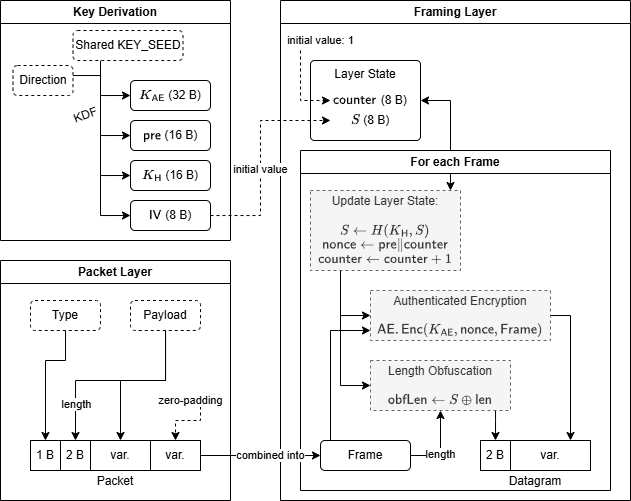
\includegraphics[width=\linewidth]{images/packet-framing.png}
    \caption[
        A visualization of \obfsfour{} framing at the sender.
    ]{
        A visualization of \obfsfour{} framing at the sender, where dashed shaded boxes correspond to subroutines, dashed unshaded boxes denote inputs, $\mathsf{AE}$ denotes the NaCl secretbox authenticated encryption scheme, and $H$ denotes the SipHash-2-4 pseudorandom function. 
    }
    \label{fig:framing}
\end{figure}

To create a packet, a packet type and the payload are required. The packet is then constructed and consists of the following:
\begin{itemize}
    \item A 1-byte packet type (corresponding to ``Payload'' or ``PrngSeed''),
    \item a 2-byte payload length in big endian format,
    \item the payload data itself, and
    \item configurable amounts of zero-padding (not included in the length calculation).
\end{itemize}

This packet is then passed on to a framing layer. While the packet layer ensures that a reliably received data stream can be decoded into separate variable-length messages with associated types, the framing layer's job is to encrypt, authenticate, and obfuscate the data.

For each direction, a counter value $\mathsf{counter}$ is initially set to 1, and a hash state $S$ is initialized to $\mathsf{IV}$.

For each frame (consisting of one or more packets) passed to the framing layer, several things occur:
\begin{enumerate}
    \item A nonce is computed as $ \mathsf{pre} \conc \mathsf{counter}$, and $\mathsf{counter}$ is incremented.
    \item One step of SipHash-2-4 in OFB mode is computed, yielding a fresh 8-byte hash state $S \gets H(K_\mathsf{H}, S)$.
\end{enumerate}

The entire packet is then encrypted using NaCl secretbox (Poly1305/XSalsa20) authenticated encryption with key $K_\mathsf{AE}$, producing a ciphertext; note that the ciphertext is longer than the packet payload, as padding and the secretbox overhead are now included.

The length of the ciphertext is then XORed with the first two bytes of the newly computed state $S$. The final datagram consists of:
\begin{itemize}
    \item A 2-byte obfuscated length field, and
    \item the AE ciphertext.
\end{itemize}

Upon receiving a packet, the receiver updates its $\mathsf{counter}$ and $S$ values, deobfuscated the length field, and decrypts the AE ciphertext. Finally, the data is passed up to the packet layer.

\paragraph{An Informal Security Analysis}

We will now discuss the achieved security guarantees by the above approach, to quickly survey possible improvements in future implementations.

The framing layer outlined above cannot, by design of the underlying Tor pluggable transport implementation, hide the length of transmitted frames from active attackers.
After the initial handshake, the connection is ``wrapped'' in the packet and framing layers, and for as long as the connections stay alive, data is passed back and forth between the local Tor client (in plaintext) and the bridge connection (encoded in packets).
If, at any point, a connection closes or raises an error (e.g. because a tag in the framing layer's AE ciphertext failed to verify), the connection is immediately closed, and a TCP FIN packet is sent by the OS as part of closing the TCP file descriptor.
This allows active attackers to choose any TCP burst after the initial handshake, leave the length field in the first two bytes unmodified, arbitrarily change the third byte (part of the 16 byte NaCl secretbox tag, ensuring a decryption failure later), and then slowly send one byte at a time. As the pluggable transport, after reading a valid length value, will wait for all data to arrive, and then verify the AE ciphertext, the total length of the AE ciphertext can be deduced by observing when the connection is closed.

This contrasts harshly with the handling of errors and invalid MAC values in the handshake procedure: There, a random delay between 1 and 60 seconds from the start of the connection is chosen as a deadline, and if a client causes an error in the handshake or does not send enough data in the first 30 seconds, the connection is closed only at this randomized deadline.

If active attackers attempt to fingerprint the connection by modifying the length value to provoke a closure of the connection (e.g. flipping the most significant bit, ensuring an invalid length), the length value is instead chosen as a random valid length between 16 to 1446 bytes. As the connection then remains blocked until the corresponding amount of AE ciphertext is received before the connection is closed, this attack cannot provoke a closure after a fixed, identifiable amount of data. The concept of ``secure closures'' of channels in general is discussed in more detail in \cite{Fenske2024}.

The main purpose of the length field obfuscation is therefore not to hide it from active attackers, or protect against manipulation (this is done by the authenticated encryption), but instead to make the protocol harder to identify. To this end, it is not clear to us, why $S$ is not instead chosen as e.g. $S \gets H(K_H, \mathsf{counter})$ to obtain a similarly secure random value to use in the XOR operation. This would remove the need for $\mathsf{IV}, S$ altogether and streamline the construction. Additionally, the \drivel{} PRF $F_1$ could be reused, reducing the number of primitives required in the protocol.

\paragraph{Design Conflicts and Conclusion}

To construct a system capable of flexible traffic shaping, it is necessary to split large messages into smaller ones, sent in sequence, as well as to pad small messages to a larger size, or even send only padding when no message is available.

The existing packet-based system in \obfsfour{} achieves exactly this, while providing authentication and side-stepping attacks from \cite{SP:AlbPatWat09}. Each packet incurs an overhead of 3 bytes plus configurable padding, and each frame (containing one or more packets, depending on the bridge configuration) adds 18 bytes.
The only precondition is a securely shared $\mathsf{KEY\_SEED}$.

It is possible to employ this system directly in \drivel{} (possibly changing the employed schemes in the framing layer to match KEM and OKEM security levels).
For example, we could first transmit $c_S \conc A_C$ without using the framing layer, and then initialize the framing layer using a key derived from the early secret $ES$. Later, we could re-initialize the framing layer using yet another key after the handshake is completed.

However, since the framing layer already aims to provide obfuscation, integrity, and confidentiality, the need for $P_C, M_C, \mathsf{MAC}_C, P_S, M_S, \mathsf{MAC}_S$ would disappear. Note that the message transcript is implicitly validated by including the $\mathsf{context}$ value when calculating $\mathsf{KEY\_SEED}$. Furthermore, it would not be necessary to encrypt $\pk_e$ at all.

We believe it to be worthwhile to modify \drivel{} accordingly, allowing almost arbitrary traffic shaping after an initial transmission of only $c_S \conc A_C$.
Conversely, this rather extensive change would require adapting the extensive $\sObfKE$ security proof for \drivel{} presented in \cite{EPRINT:GRSV25}.

This approach is visualized in \cref{fig:modified-drivel-framing}, an adaptation of \cite[Figure~6]{EPRINT:GRSV25}. Let $FL$ denote the framing layer presented above. Then $FL.\mathsf{Rekey}(k)$ indicates that the framing layer is reinitialized using $k$ as the $\mathsf{KEY\_SEED}$ value following the process outlined above.

In addition, we took the opportunity to propose a simplification of the calculation of PRF values in order to optimize memory performance:
As $F_1$ is implemented as \textsf{HDKF-Expand}, its state after digesting part of its input cannot be reused for further calls to $F_1$ (due to e.g. the string constants used for domain separation) and its entire input must be re-hashed when requesting multiple output blocks.
Both shortcomings can be circumvented by instead pre-hashing long inputs without appending a string constant. This hash state could also be reused when more inputs are desired in the later stages of the protocol.

To this end, we introduce a hash function $\mathbf{H}$ and replace the inputs to $F_1$ appropriately. This approach is similar in spirit to e.g. the calculation of the transcript hash in TLS 1.3 by keeping a running hash value \cite[Section~4.4.1]{rfc8446}.

\begin{figure}
    % \begin{minipage}[t]{\textwidth}
	\hfill
	\pseudocode[codesize=\footnotesize,jot=-1mm]{%
		\textbf{Server key generation/setup} \\
		\nodeid \getsr \bin^{\nodeidlen} \\
		(\pk_S, \sk_S) \getsr \OKEM.\kgen() \\
		\pstate.\macregister \gets \emptyset \\
		\text{return } ((\pk_S, \nodeid), (\sk_S, \nodeid), \pstate)
	}
	\hspace*{0.8cm}
% \end{minipage}

% \vspace{0.5em}

% \hspace*{-0.2in}
\centering
\scalebox{0.9}{%
\begin{tikzpicture}
	% Set the X coordinates of the client, server, and arrows
	\edef\ClientX{0}

	\edef\ArrowLeft{3}
	\edef\ArrowRight{13}
	\edef\ServerX{16.5}
	\edef\ServerLeftTextwidth{10.5cm} % width of server-side text, when left-aligned

	% Set the starting Y coordinate
	\edef\Y{0}

	% Draw header boxes
	\node [rectangle,draw,inner sep=5pt,right] at (\ClientX,\Y) {\textbf{Client}};
	\node [rectangle,draw,inner sep=5pt,left] at (\ServerX,\Y) {\textbf{Server}};
	
	\NextLine[0.4]
	\ClientAction[gray,font=\small]{\hspace{1.5cm}knows $(\pk_S, \nodeid)$}
	\ServerAction[gray,font=\small]{knows $(\sk_S, \nodeid)$\hspace{1.5cm}\null}
	\NextLine[1.1]
	
	\ClientAction{$(\pk_e, \sk_e) \getsr \KEM.\kgen()$} 
	\NextLine
	\ClientAction{$(c_S, K_S) \getsr \OKEM.\encaps(\pk_S)$}
	\NextLine
	\ClientAction{$ES \gets \funComb(\nodeid, K_S)$}
	\NextLine
	\ClientAction{$\mathsf{protoID} \gets \textlit{Drivel}$}
	\NextLine
	\ClientAction{\highlightbox{$\mathsf{context}_1 \gets \mathsf{protoID} \conc \pk_S \conc c_S$}}
	\NextLine
	\ClientAction{\highlightbox{$A_C \gets \funPRF(ES, \mathbf{H}(\mathsf{context}_1) \conc \textlit{:authc})$}}
	\NextLine
	\ClientAction{\highlightbox{$\mathsf{KEY\_SEED}_1 \gets \funPRF(ES, \mathbf{H}(\mathsf{context}_1) \| \textlit{:key\_extract\_1})$}}
	%%%%%%%%%%%%%%%%%%%%%%%%%%%%%%%%%%%%%%%%%%%%%%%%%%%%%%%%%%%%%%%%%%%%%%%%%%%%%%%%%%%%%%%%%%%%%%%%%%%%%%%
	\NextLine[2]
	\ClientToServer{\highlightbox{$\mathsf{msg}_C' = c_S \conc A_C$}}{}
	\NextLine
    %%%%%%%%%%%%%%%%%%%%%%%%%%%%%%%%%%%%%%%%%%%%%%%%%%%%%%%%%%%%%%%%%%%%%%%%%%%%%%%%%%%%%%%%%%%%%%%%%%%%%%%

    % Server verifies A_C and can start with dummy data
	\ServerActionLeft{$K_S \gets \OKEM.\decaps(\sk_S, c_S)$}
	\NextLine
	\ServerActionLeft{$ES \gets \funComb(\nodeid, K_S)$}
	\NextLine
	\ServerActionLeft{$\mathsf{protoID} \gets \textlit{Drivel}$}
	\NextLine
	\ServerActionLeft{\highlightbox{$\mathsf{context}_1 \gets \mathsf{protoID} \conc \pk_S \conc c_S$}}
	\NextLine
	\ServerActionLeft{\highlightbox{if $\funPRF(ES, \mathbf{H}(\mathsf{context}_1) \conc \textlit{:authc}) \neq A_C$: $\texttt{break}$}}
	\NextLine
	\ServerActionLeft{if \highlightbox{$A_C$}$ \in \pstate.\macregister$: $\texttt{break}$}
	\NextLine
	\ServerActionLeft{$\pstate.\macregister \gets \pstate.\macregister \cup $\highlightbox{$\{A_C\}$}}
	\NextLine
	\ServerActionLeft{\highlightbox{$\mathsf{KEY\_SEED}_1 \gets \funPRF(ES, \mathbf{H}(\mathsf{context}_1) \| \textlit{:key\_extract\_1})$}}
    %%%%%%%%%%%%%%%%%%%%%%%%%%%%%%%%%%%%%%%%%%%%%%%%%%%%%%%%%%%%%%%%%%%%%%%%%%%%%%%%%%%%%%%%%%%%%%%%%%%%%%%

    % Rekeying 1
    \NextLine
	\PhaseBreak{}{}
	\NextLine
    \ClientAction{\highlightbox{$FL.\mathsf{Rekey}(\mathsf{KEY\_SEED}_1)$}}
    \ServerAction{\highlightbox{$FL.\mathsf{Rekey}(\mathsf{KEY\_SEED}_1)$}}
    \NextLine[0.5]
	%%%%%%%%%%%%%%%%%%%%%%%%%%%%%%%%%%%%%%%%%%%%%%%%%%%%%%%%%%%%%%%%%%%%%%%%%%%%%%%%%%%%%%%%%%%%%%%%%%%%%%%

    % Start sending arbitrary data
	\ServerToClient[dashed,->]{}{}
	\ServerAction{\highlightbox{send arbitrary data}}
    %%%%%%%%%%%%%%%%%%%%%%%%%%%%%%%%%%%%%%%%%%%%%%%%%%%%%%%%%%%%%%%%%%%%%%%%%%%%%%%%%%%%%%%%%%%%%%%%%%%%%%%
    \NextLine[2]
	\ClientToServer{\highlightbox{$\mathsf{msg}_C'' = \pk_e$}}{}
	\NextLine
	%%%%%%%%%%%%%%%%%%%%%%%%%%%%%%%%%%%%%%%%%%%%%%%%%%%%%%%%%%%%%%%%%%%%%%%%%%%%%%%%%%%%%%%%%%%%%%%%%%%%%%%

    % Server parses rest of message and replies
    \ServerActionLeft{$(c_e, K_e) \getsr \KEM.\encaps(\pk_e)$}
	\NextLine
	\ServerActionLeft{$ES' \gets \funPRF(ES, \textlit{:derive\_key})$ ; $FS \gets \funComb(ES', K_e)$}
	\NextLine
	\ServerActionLeft{\highlightbox{$\mathsf{context}_2 \gets \mathsf{context}_1 \conc \pk_e \conc c_e$}}
	\NextLine
	\ServerActionLeft{$\mathsf{KEY\_SEED}_2 \gets \funPRF(FS, $\highlightbox{$\mathbf{H}(\mathsf{context}_2)$}$ \conc \textlit{:key\_extract\_2})$}
	\NextLine
	\ServerActionLeft{$\mathsf{auth} \gets \funPRF(FS, $\highlightbox{$\mathbf{H}(\mathsf{context}_2)$}$ \conc \textlit{:server\_mac})$}
	%%%%%%%%%%%%%%%%%%%%%%%%%%%%%%%%%%%%%%%%%%%%%%%%%%%%%%%%%%%%%%%%%%%%%%%%%%%%%%%%%%%%%%%%%%%%%%%%%%%%%%%
	\NextLine[1.5]
	\ServerToClient{\highlightbox{$\mathsf{msg}_S = c_e \conc \mathsf{auth}$}}{}
    %%%%%%%%%%%%%%%%%%%%%%%%%%%%%%%%%%%%%%%%%%%%%%%%%%%%%%%%%%%%%%%%%%%%%%%%%%%%%%%%%%%%%%%%%%%%%%%%%%%%%%%

    \NextLine
	\ClientAction{$K_e \gets \KEM.\decaps(\sk_e, c_e)$}
	\NextLine
	\ClientAction{$\mathsf{protoID} \gets \textlit{Drivel}$}
	\NextLine
	\ClientAction{$ES' \gets \funPRF(ES, \textlit{:derive\_key})$ ; $FS \gets \funComb(ES', K_e)$}
	\NextLine
	\ClientAction{\highlightbox{$\mathsf{context}_2 \gets \mathsf{context}_1 \conc \pk_e \conc c_e$}}
	\NextLine
	\ClientAction{$\mathsf{KEY\_SEED}_2 \gets \funPRF(FS, $\highlightbox{$\mathbf{H}(\mathsf{context}_2)$}$ \| \textlit{:key\_extract\_2})$}
	\NextLine
	\ClientAction{if $\funPRF(FS, $\highlightbox{$\mathbf{H}(\mathsf{context}_2)$}$ \conc \textlit{:server\_mac}) \neq \mathsf{auth}$: $\texttt{break}$}
    %%%%%%%%%%%%%%%%%%%%%%%%%%%%%%%%%%%%%%%%%%%%%%%%%%%%%%%%%%%%%%%%%%%%%%%%%%%%%%%%%%%%%%%%%%%%%%%%%%%%%%%

    % Rekeying 2
    \NextLine
	\PhaseBreak{}{}
	\NextLine
    \ClientAction{\highlightbox{$FL.\mathsf{Rekey}(\mathsf{KEY\_SEED}_2)$}}
    \ServerAction{\highlightbox{$FL.\mathsf{Rekey}(\mathsf{KEY\_SEED}_2)$}}
\end{tikzpicture}
}

    \caption[
        The modified \drivel{} protocol, simplified to take advantage of a framing layer.
    ]{
        The modified \drivel{} protocol, simplified to take advantage of a framing layer.
        $\OKEM$ is an OKEM satisfying $\indcca, \sprcca$ security, and ciphertext uniformity.
        $KEM$ is an $\indonecca$-secure KEM.
        $FL$ is a framing layer similar to the one described in \cref{sssec:variant-framing}.
        $F_1$ is a PRF and $F_2$ is a dual PRF.
        $\mathbf{H}$ is a collision-resistant hash function.
        Core differences to the \drivel{} protocol from \cite[Figure~6]{EPRINT:GRSV25} are highlighted in blue boxes.
        Messages are easily parsed due the the packet layer providing boundaries and the fixed-length components.
        A dashed arrow represents the option to send an arbitrary amount of uniformly random bits for the purpose of traffic shaping, e.g. by sending packets consisting only of padding.
        Dotted lines delimit the framing layer phases between $FL.\mathsf{Rekey}$ operations.
    }
    \label{fig:modified-drivel-framing}
\end{figure}

\paragraph{Note to Implementers and Future Work}

Should readers choose to implement or improve upon this proposed variant of \drivel{}, we encourage them to also consider the following items:

\begin{itemize}
    \item Calculating $\mathbf{H}(\mathsf{context}_2)$ can be done efficiently by reusing the hash state after digesting $\mathsf{context}_1$, avoiding the need to hash $\mathsf{context}_1$ twice. The hash outputs can be reused for two invocations of $F_1$ each time.
    
    \item This variant does not have a security proof like \drivel{}, and producing one would require formalizing the guarantees provided by the framing layer.

    \item As this thesis focuses on the key exchange phase, we did not propose improvements to the framing layer. However, previous work in this space exists \cite{Fenske2024} and should be considered to improve the framing layer from \obfsfour{}.

    \item Attention should be paid in particular to preventing modifications to the length fields (e.g. by authenticating them using fixed-length fields), and to handling errors consistently as discussed in the security analysis above and in \cite[Section~3.3]{Fenske2024}.

\end{itemize}

\section{Core Architecture} \label{sec:impl-architecture}
% TODO
% \Cref{sec:impl-architecture} describes how the protocol design was mapped to actual software components, including noteworthy architectural changes and cryptographic interfaces.

After discussing the \drivel{} protocol (and our proposed changes) in \cref{sec:protocol-design}, we now take a closer look at how we implemented the \drivel{} protocol based on the existing \obfsfour{} implementation in the lyrebird repository.

Recall the general structure of the repository into four main Go modules from \cref{sec:tech-stack}. Here, we consider two of these modules in more detail: the \texttt{internal} module, which was significantly refactored and extended, and the \texttt{transports/drivel} module containing all \drivel{}-specific code.

\paragraph{Building a KEM and OKEM from the \texttt{internal/x25519ell2} Module}

In the implementation of \obfsfour{}, only one method of key exchange is available: Customized Diffie-Hellman key exchange on the elliptic curve x25519, possibly using the \textsf{Elligator2} encoding on the curve points transmitted over the wire.

Post-quantum key-exchange algorithms are almost universally specified using the syntax of KEMs. In order to compare \drivel{} performance in the traditional setting with its performance using post-quantum KEMs, we have extended the \texttt{internal/x25519ell2} module to implement a KEM and a filter-encode obfuscator performing \textsf{Elligator2}. \Cref{fig:impl-x25519-kem} shows pseudocode illustrating the usage of the module by \obfsfour{} (through its use of the \texttt{common/ntor} module), alongside the construction of our x25519 KEM.

As our goal is simply to show how the KEM construction was extracted from the existing code, we omit the full definition of \obfsfour{} here. Suffice to say, the protocol involves one static keypair $\pk_\mathsf{id}, \sk_\mathsf{id}$ (the public key is part of the bridge information) and two ephemeral keypairs generated during the handshake procedure. The static keypair has no encodings applied to the public key (as it is transmitted out-of-band), while the ephemeral keypairs also have obfuscated public keys. When all required values are available, methods $\mathsf{ServerHandshake}, \mathsf{ClientHandshake}$ are executed to compute shared secrets which in turn are used to authenticate and finalize the handshake.

Readers should note that, although the construction is similar in spirit to the DHKEM construction \cite[Section~4.1]{rfc9180}, this KEM has minor differences in the derivation of its shared secret. Instead, the focus was on staying as close as possible to the construction used in \obfsfour{}, in order to offer a fair comparison between the two pluggable transport constructions when targeting traditional security.

Unlike in the \obfsfour{} protocol, the newly constructed KEM has what initially appear to be slightly different semantics to generate the obfuscated ciphertext $\hat \pk$:
In \obfsfour{} and its method $\mathsf{NewKeypair}$, the value $u$ determined by $\sk$ is passed directly to $\mathsf{uToRepresentative}$ whereas in the KEM, additional serialization ($\mathsf{Bytes}$) and deserialization ($\mathsf{SetBytes}$) takes place before $\mathsf{uToRepresentative}$ is invoked.
We have experimentally verified that this does not change $u$ and that the same $\hat \pk$ values are generated with both approaches, given the same randomness $t$.
Finally, the randomness $t$ is not taken from the hash function output used to set $\sk$, but rather generated securely on-the-fly. It is merely used for padding with two random bits, and to pick the sign of the curve point's y-coordinate at random as suggested in \cite{elligatorExplicitFormulas}.

\begin{figure}
    \begin{pchstack}[boxed, center, space=0.5em]

    \begin{pcvstack}[space=0.05em]
    % obfs4 usage via common/ntor
    \procedure[linenumbering]{Initialization}{
        \pclinecomment{$\pk_\mathsf{id}$ is part of the bridge information:} \\
        (\pk_\mathsf{id},\sk_\mathsf{id}) \getsr \mathsf{NewKeypair}(\mathsf{ell2}=0) \\
        \pclinecomment{upon the start of a new handshake:} \\
        (\pk_c,\sk_c) \getsr \mathsf{NewKeypair}(\mathsf{ell2}=1) \\
        (\pk_s,\sk_s) \getsr \mathsf{NewKeypair}(\mathsf{ell2}=1)
    }

    \procedure[linenumbering]{$\mathsf{NewKeypair}(\mathsf{ell2} \in \bin)$}{
        \pcdo \\
        \t  r \getsr \bin^{256} \\
        \t  d \gets \operatorname{\mathsf{SHA2-512}}(r) \\
        \t  \sk \gets \mathsf{firstBytes}(d,32) \\
        \t  \pcif \mathsf{ell2} = 1 \pcthen \\
        \t  \t  t \gets \mathsf{lastBytes}(d,1) \\
        \t  \t  \pclinecomment{inlined ScalarBaseMult(\sk, t)} \\
        \t  \t  u \gets \mathsf{scalarBaseMultDirty}(\sk) \\
        \t  \t  \pk \gets \mathsf{Bytes}(u) \\
        \t  \t  \hat \pk \gets \mathsf{uToRepresentative}(u, t) \\
        \t  \t  \pcif \pk \neq \bot \pcthen \\
        \t  \t  \t  \pcreturn (\pk, \hat \pk, \sk) \\
        \t  \t  \pcendif \\
        \t  \pcelse \\
        \t  \t  \pk \gets \mathsf{curve25519}.\mathsf{ScalarBaseMult}(\sk) \\
        \t  \t  \pcreturn (\pk, \bot, \sk) \\
        \t  \pcendif \\
        \pcwhile \pctrue
    }
   
    \procedure[lnstart=4,linenumbering]{$\mathsf{ServerHandshake}(\hat \pk_c, (\pk_s, \sk_s), (\pk_\mathsf{id},\sk_\mathsf{id}))$}{
        \pk_c \gets \mathsf{RepresentativeToPublicKey}(\hat \pk_c) \\
        K_1 \gets \mathsf{curve25519}.\mathsf{ScalarMult}(\sk_s, \pk_c) \\
        K_2 \gets \mathsf{curve25519}.\mathsf{ScalarMult}(\sk_\mathsf{id}, \pk_c) \\
        \pcif K_1 = 0 \lor K_2 = 0 \pcthen \pcabort \pcendif
    }
    
    \procedure[lnstart=4,linenumbering]{$\mathsf{ClientHandshake}((\pk_c, \sk_c), \hat \pk_s, \pk_\mathsf{id})$}{
        \pk_s \gets \mathsf{RepresentativeToPublicKey}(\hat \pk_s) \\
        K_1 \gets \mathsf{curve25519}.\mathsf{ScalarMult}(\sk_c, \pk_s) \\
        K_2 \gets \mathsf{curve25519}.\mathsf{ScalarMult}(\sk_c, \pk_\mathsf{id}) \\
        \pcif K_1 = 0 \lor K_2 = 0 \pcthen \pcabort \pcendif
    }
    \end{pcvstack}

    \begin{pcvstack}[space=0.05em]
    % KEM components
    \procedure[linenumbering]{$\KEM.\kgen()$}{
        r \getsr \bin^{256} \\
        d \gets \operatorname{\mathsf{SHA2-512}}(r) \\
        \sk \gets \mathsf{firstBytes}(d,32) \\
        u \gets \mathsf{scalarBaseMultDirty}(\sk) \\
        \pk \gets \mathsf{Bytes}(u) \\
        \pcreturn (\pk, \sk)
    }
   
    \procedure[lnstart=4,linenumbering]{$\KEM.\encaps(\pk)$}{
        \pk_e, \sk_e \getsr \kgen() \\
        K \gets \mathsf{curve25519}.\mathsf{ScalarMult}(\sk_e, \pk) \\
        \pcif K = 0 \pcthen \\
        \t  \pcabort \\
        \pcendif \\
        \pcreturn (c=\pk_e, K)
    }
    
    \procedure[lnstart=9,linenumbering]{$\KEM.\decaps(\sk, c)$}{
        u \gets \mathsf{SetBytes}(c) \\
        K \gets \mathsf{curve25519}.\mathsf{ScalarMult}(\sk, \mathsf{Bytes}(u)) \\
        \pcif K = 0 \pcthen \\
        \t  \pcabort \\
        \pcendif \\
        \pcreturn K
    }

    % FEO components
    \procedure[linenumbering]{$E.\filterpk(\pk)$}{
        \pclinecomment{no restriction on $\pk$ to encapsulate against} \\
        \pcreturn \pctrue
    }
    
    \procedure[lnstart=3,linenumbering]{$E.\encodectxt(c)$}{
        t \getsr \bin^{8} \\
        u \gets \mathsf{SetBytes}(c) \\
        \hat \pk \gets \mathsf{uToRepresentative}(u, t) \\
        \pclinecomment{$\hat \pk$ is $\bot$ for 50\% of all values of $c$} \\
        \pcreturn \hat \pk
    }
    
    \procedure[lnstart=5,linenumbering]{$E.\decodectxt(\hat c)$}{
        \pcreturn \mathsf{RepresentativeToPublicKey}(\hat c)
    }
    \end{pcvstack}

\end{pchstack}
    \caption[
        Pseudocode illustrating the x25519 KEM and filter-encode obfuscator added to the \texttt{internal/x25519ell2} module.
    ]{
        Pseudocode illustrating the x25519 KEM $\KEM$ and a filter-encode obfuscator $E$, both added to the \texttt{internal/x25519ell2} module.
        The left-hand side of the figure shows the usage of the x25519 module by \obfsfour{}, while the right-hand side defines a KEM and obfuscator for use in \drivel{}.
        The aborts identify insecure secrets caused by low-order public keys.
        We use $\mathsf{firstBytes}(x, \ell), \mathsf{lastBytes}(x, \ell)$ to denote selecting the first or last $\ell$ bytes of $x$, respectively.
        $\mathsf{curve25519}$ denotes the submodule of \texttt{golang.org/x/crypto} by the same name, all other functions are from the lyrebird repository's \texttt{internal/x25519ell2} and \texttt{common/ntor} modules.
    }
    \label{fig:impl-x25519-kem}
\end{figure}

\paragraph{Adding Crypto-Agility to the \texttt{internal} Module}

Observing the current need for post-quantum key exchange, combined with the increasing deployment of newly standardized algorithms, it seems prudent to implement flexibility in the utilized key exchange schemes. Being able to exchange cryptographic algorithms is often called ``being crypto-agile''.

To this end, the \drivel{} implementation contains string constants identifying the desired KEM and OKEM. The data structures for the schemes are then loaded at runtime based on these strings.
The schemes are identified by the following naming convention:
\begin{itemize}
    \item The string "x25519" refers to the unobfuscated, newly implemented KEM from \cref{fig:impl-x25519-kem},
    \item all other strings denote \texttt{liboqs} KEMs, and
    \item any KEM with a corresponding filter-encode obfuscator can be used to request an OKEM under the KEM name prefixed with ``FEO-'', e.g. ``FEO-x25519'' would denote $\feo[\KEM, E]$ using the components from \cref{fig:impl-x25519-kem}.
\end{itemize}

Note that some ``FEO-'' schemes may in fact simply be the unmodified KEM (the code uses a \texttt{nil} encoder reference), but the naming convention ensures that the name of a scheme clearly separates KEMs from OKEMs. Additionally, as discussed above in \cref{sec:parameters}, some KEMs and OKEMs available from \texttt{liboqs} are disabled to limit the number of test cases and enable some optimizations with regards to buffer sizes.

Due to the different origin of these KEM and OKEM implementations, and the lack of an abstract standardized KEM interface in Go suitable for these constructions, we added several new submodules to \texttt{internal}:
\begin{itemize}
    \item \texttt{internal/cryptodata} offers a \texttt{CryptoData} type which holds a byte string. Conversions to and from hexadecimal representation are implemented here, as well as assertions checking the size of these byte strings. The latter is enforced as part of the constructor. This helps to prevent accidental changes to the size of these objects, and ensures that we are always working with fixed-length strings. Internally, these objects are simply Go byte slices but our type restricts the possible operations to a minimum.

    \item \texttt{internal/kems} and \texttt{internal/okems} are two submodules that implement KEM and OKEM interfaces, as well as data types for serializable public keys, private keys, keypairs, ciphertexts and shared secrets. While these submodules contain very similar code, the differentiation ensures that e.g. KEM ciphertexts can only be used in a context where OKEM ciphertexts are required by explicitly casting from one type to another. Again, this helps the readability and prevents certain implementation mistakes.

    \item \texttt{internal/cryptofactory} contains the final additional submodule and constitutes our main contribution to the \texttt{internal} module. Its job is to expose a list of supported KEMs and OKEMs for test purposes, as well as two constructors \texttt{NewKem} and \texttt{NewOkem} allowing for the construction of a scheme based only on its name as described above. Several nested submodules implement specific functionality:
    \begin{itemize}
        \item \texttt{internal/cryptofactory/encoding\_classic\_mceliece} implements a filter-encode-obfuscator for ``Classic-McEliece-6960119'',
        \item \texttt{internal/cryptofactory/encoding\_hqc} implements filter-encode-obfuscators for all three HQC parameter sets,
        \item \texttt{internal/cryptofactory/encoding\_kemeleon} implements the ``Non-Rejection Sampling Variant'' of the filter-encode-obfuscators for ML-KEM from \cite{irtf-cfrg-kemeleon-00},
        \item \texttt{internal/cryptofactory/filter\_encode} defines an interface for these obfuscators and implements the generic FEO transformation from \cref{def:filter-encode-okem}, and, finally,
        \item \texttt{internal/cryptofactory/oqs\_wrapper} implements a thin wrapper which makes the \texttt{liboqs} KEM interface compatible with our interface defined in \texttt{internal/kems}\footnote{Our interface differs from the existing \texttt{liboqs} and Go interfaces in that it uses the data types introduced in \texttt{internal/cryptodata}, more closely matches the KEM syntax used in this thesis, and provides fewer pieces of information about the KEM.}.
    \end{itemize}
\end{itemize}

Each of the filter-encode obfuscators is covered with unit tests to check that ciphertexts are recovered without change after encoding and subsequent decoding. Our theoretical first-keygen and first-encaps success probabilities are verified, and some sanity-checks are performed to validate the encoding outputs. All available KEMs and OKEMs are also tested for their correctness and benchmarked for their performance as part of the \texttt{internal/cryptofactory} submodule.

\paragraph{Notable Differences between \texttt{transports/drivel} and \texttt{transports/obfs4}}

Although the \texttt{transports/drivel} module started out as a copy of \texttt{transports/obfs4}, multiple conceptual changes were made during the course of this thesis.

While \texttt{transports/obfs4} depends on \texttt{common/ntor} to implement the main cryptography beyond obfuscation, this functionality is now provided instead by \texttt{transports/drivel/drivelcrypto}. This functionality is now less spread out through the repository. Test cases from the \texttt{common/ntor} module were copied and extended as needed.
Functionality of this new submodule includes:
\begin{itemize}
    \item the generation and (de-)serialization of $\mathsf{NodeID}$,
    \item the definition of types for the values $\mathsf{auth}$ and $\mathsf{KEY\_SEED}$,
    \item constant-time comparisons for $\mathsf{MAC_C}, \mathsf{MAC_S}$ and $\mathsf{auth}$,
    \item the derivation of $\mathsf{auth}$ and $\mathsf{KEY\_SEED}$ after all protocol messages have been parsed and authenticated (as this functionality is shared between client and server),
    \item functions to calculate $\mathsf{M_C}, \mathsf{M_S}, \mathsf{MAC_C}, \mathsf{MAC_S}$ more easily,
    \item all relevant string constants for these procedures,
    \item implementations for $F_1, F_2$ and the symmetric encryption scheme $SE$
\end{itemize}

The framing layer \texttt{transports/drivel/framing} and packet layer \texttt{transports/drivel/packet.go} are essentially unchanged compared to \texttt{transports/obfs4}.

The main protocol functionality is implemented in \texttt{transports/drivel/handshake.go}, handling state objects persisted through the course of a connection, and implementing functions to initialize this state, parse messages, and generate responses.
Sitting between the low-level cryptography primitives and the higher-level handshake process, this file was significantly adapted from its predecessor \texttt{transports/obfs4/handshake\_ntor.go}, and now employs the newly added data types from \texttt{internal}.
One noteworthy change in particular is that the sizes of public keys, private keys, ciphertexts and shared secrets is not statically known anymore as the schemes are only selected at runtime. This enables us to provide a single client binary capable of connecting to multiple bridges, each using different KEM/OKEM combinations. Instead of hardcoding sizes, we respect sizes reported by \texttt{liboqs} at runtime to further reduce the changes required to switch out a KEM or OKEM.
This approach led to the addition of some runtime calculations of possible padding values and expected sizes of message components in a new \texttt{lengthDetails} object.

As a final change, we consider \texttt{transports/drivel/drivel.go} and \texttt{transports/drivel/statefile.go} which handle the high-level protocol functionality such as parsing arguments, and loading saved bridge information, as well as constructing the connection used for later data transfer after the handshake phase is completed.
A significant change here concerned the passing of bridge information between the client's configuration file and the pluggable transport implementation: The Tor ecosystem requires all pluggable transports to implement a SOCKS proxy setup. The content of the client's configuration is then sent to its local SOCKS proxy via the username and password fields (as the proxy is only available locally, there is no actual authentication) and the bridge IP is provided as a target address. In \texttt{transports/obfs4}, this configuration contains the $\mathsf{NodeID}$ as well as the server's static public key $\pk_S$. However, for post-quantum OKEMs the size of this public key exceeds the limit of SOCKS username and password sizes, which may have a combined length of at most 510 bytes. This issue has already been noted by David Fifield in the context of the Snowflake pluggable transport \cite{torprojectSnowflakeBridge}. While possible solutions have been discussed in the Tor Project, there is (at the time of writing) no standardized solution as part of the Tor ecosystem.

To circumvent this limitation, clients are now required to:
\begin{itemize}
    \item add the so-called ``bridge-line'' to their configuration file (as for \obfsfour{}), containing (among other things) the name of the pluggable transport, IP and port of the bridge, and the $\mathsf{NodeID}$, but now also
    \item download a public key file called \texttt{drivel\_key-<KEYID>} containing $\pk_S$ in JSON format, where \texttt{<KEYID>} is a prefix of $\mathsf{NodeID}$. This file is created in the correct format by the bridge upon starting.
\end{itemize}

As the configuration is now considerably shorter, it can be transmitted via the SOCKS fields, and the pluggable transport can load the public key corresponding to $\mathsf{NodeID}$ from the disk.

Additionally, the public key file contains the names of the KEM and OKEM schemes that the bridge is configured to use. This ensures interoperability and allows clients to use different schemes depending on the selected bridge.

\section{Deployment Guide} \label{sec:deployment}

Note that this setup procedure is not geared towards end users, and a more user-friendly procedure is required for wide-spread deployment.
However, since this involves multiple changes to the current distribution mechanisms and \drivel{} may be further adapted before then, we believe that further improvements are premature at this point.

In order to deploy our implementation of \drivel{} as a Tor pluggable transport, we recommend the following procedure:
\begin{enumerate}
    \item Clone our fork of the lyrebird repository\footnote{See \url{https://gitlab.ethz.ch/himarc/lyrebird-pq-obfs}} into a new directory called ``lyrebird''
    
    \item Clone the official Tor repository containing recommended container files from the ``docker-obfs4-bridge'' repository\footnote{See \url{https://gitlab.torproject.org/tpo/anti-censorship/docker-obfs4-bridge}} into another directory called ``docker'' next to the one just created
    
    \item Adapt the files of ``docker-obfs4-bridge'' to match the contents of the corresponding files in the \texttt{docker/bridge} folder in our analysis repository\footnote{See \url{https://gitlab.ethz.ch/himarc/thesis-quantumsafe-fep}}. This changes the build process to not use the official lyrebird repository but instead copy the contents of a local ``lyrebird'' folder, install all necessary build dependencies and perform the build. Additionally, the bridge-line format requires minor changes to the ``get-bridge-line'' and ``start-tor.sh'' files.

    \item For production use, perform the following additional steps:
    \begin{enumerate}
        \item Remove the file \texttt{wrapper.sh}, and delete the following lines from the file \texttt{Dockerfile}
        \begin{lstlisting}
COPY docker/bridge/wrapper.sh /usr/bin/wrapper.sh
RUN chmod +x /usr/bin/wrapper.sh
        \end{lstlisting}

        \item Replace ``/usr/bin/wrapper.sh'' by ``/usr/bin/lyrebird'' in \texttt{start-tor.sh}

        \item Re-enable the publication of server descriptors and the bridge distribution by removing the following lines from \texttt{start-tor.sh}:
        \begin{lstlisting}
PublishServerDescriptor 0
BridgeDistribution none
        \end{lstlisting}
    \end{enumerate}
    \label{bul:prod-use-changes}

    \item The rest of the setup requires merely setting the correct environment variables and building the docker container. This is well described in the official Tor guide\footnote{See \url{https://community.torproject.org/relay/setup/bridge/docker/}}, which references a \texttt{docker-compose.yml} file. Simply download this file, place it next to the two folders created above and replace the line ``image: thetorproject/obfs4-bridge:latest'' by the following three lines:
    \begin{lstlisting}
build:
  context: .
  dockerfile: docker/bridge/Dockerfile
    \end{lstlisting}

    \item Additionally, make sure that you set the environment variable ``TOR\_PT\_SERVER\_TRANSPORT\_OPTIONS'' in the \texttt{docker-compose.yml} file. Specify the variables ``kem-name'' and ``okem-name'' to configure the schemes used by \drivel{}. An example is:
    \begin{lstlisting}
TOR_PT_SERVER_TRANSPORT_OPTIONS="drivel:kem-name=ML-KEM-512;drivel:okem-name=FEO-Classic-McEliece-348864"
    \end{lstlisting}

    \item Finally, start the tor bridge using the command \texttt{docker-compose up -d} in the same directory as \texttt{docker-compose.yml}
\end{enumerate}

To connect, clients then require the information output by ``get-bridge-line'' in the running docker container, and all JSON files in the folder \texttt{/var/lib/tor/pt\_state/} whose name starts with \texttt{drivel\_key-}.

For clients, the same procedure to compile the lyrebird repository can be reused. Additionally, an installation of Tor is required, the bridge-line should be added to the \texttt{torrc} file and the public key file should be placed into the folder \texttt{/var/lib/tor/pt\_state}. This procedure is simpler as the format of bridge-lines does not have to be accounted for, and the main change is the use of a locally compiled lyrebird binary.

An example of such a setup can be seen in our analysis repository, which is configured to run both a bridge and a client container locally in a very similar manner, albeit with more debugging options and automatic transfer of the bridge-line and public keys, thus the changes described above in \cref{bul:prod-use-changes}.

\section{Challenges and Lessons Learned} \label{sec:challenges-learnings}

To summarize, the implementation of \drivel{} to the point of working test deployments, reusing existing tools for \obfsfour{} was a success.

Some modifications to the protocol may prove promising in the future, both in terms of flexibility and performance, but also for obfuscation. Nonetheless, we believe this implementation to provide a valuable starting point for future work.

In the following, we list some concrete implementation challenges experienced during this thesis:
\begin{itemize}
    \item KEM public keys were too large to use the XOR symmetric encryption as outlined in \cite{EPRINT:GRSV25}, as the HKDF could not provide enough key material. This required the use of AES-CTR.

    \item KEM public keys were also too large to send as part of the bridge-line in the SOCKS fields. We therefore added public key files, which are generated by the bridge and must also be sent to the client.

    \item Due to the crypto-agility introduced, the client now needs to know ahead of time, what KEM and OKEM scheme the server is configured to use. A negotiation as part of the handshake was out-of-scope for this thesis. Thus, we made servers schemes configurable via the ``TOR\_PT\_SERVER\_TRANSPORT\_OPTIONS'' environment variable and saved the names of schemes (following our naming convention) into the public key file distributed alongside the bridge-line. Clients, upon receiving $\mathsf{NodeID}$ via the SOCKS fields then load the correct file, and are now able to initialize the KEM and OKEM accordingly.

    \item This thesis contains one of the first implementations of ML-Kemeleon. One previous implementation \cite{ct-kemeleon} did not implement the \texttt{SamplePreimage} function from the Internet-Draft, and another \cite{jmwample-kemeleon} only had partial test cases for this function, and did not correctly sample uniformly random outputs. We implemented comprehensive tests, and verified the expected output distribution of \texttt{SamplePreimage}. Necessary changes to the Internet-Draft were identified in the process, and the draft authors, as well as the authors of the two previous implementations were informed of our findings.

    \item An unaddressed issue is the need to hash certain pieces of data multiple times over the course of the protocol due to the design of \drivel{}. In fact, our implementation does suffer from high memory usage compared to \obfsfour{}, and optimizations to reduce that would be beneficial. As the keys and suffixes used in HKDF change, the previous results cannot easily be reused for future calculations. In particular, requesting multiple output blocks from $F_1$ would quickly become quite costly. We consequently chose our output lengths appropriately to avoid this effect and suggested an alternative approach in \cref{sssec:variant-framing}.
\end{itemize}

In order for software to remain flexible for future adaptations, it is beneficial to avoid hardcoding specific algorithms. A modular approach where components such as encryption, PRFs, and KEMs can be easily exchanged ensures that future developments cause fewer changes to the overall system. Even apparently harmless limitations such as SOCKS field lengths can constitute integration barriers in the future.

As a final note of this chapter, the highly transparent and open-source development of the Tor project enabled us to focus directly on making material changes to an existing implementation. The open ecosystem was extremely valuable and enabled us to contribute more easily.
